\hypertarget{interface_t_p_parameter_axis_style}{
\section{TPParameterAxisStyle Class Reference}
\label{interface_t_p_parameter_axis_style}\index{TPParameterAxisStyle@{TPParameterAxisStyle}}
}
{\tt \#import $<$TPParameterAxisStyle.h$>$}

Inheritance diagram for TPParameterAxisStyle::\begin{figure}[H]
\begin{center}
\leavevmode
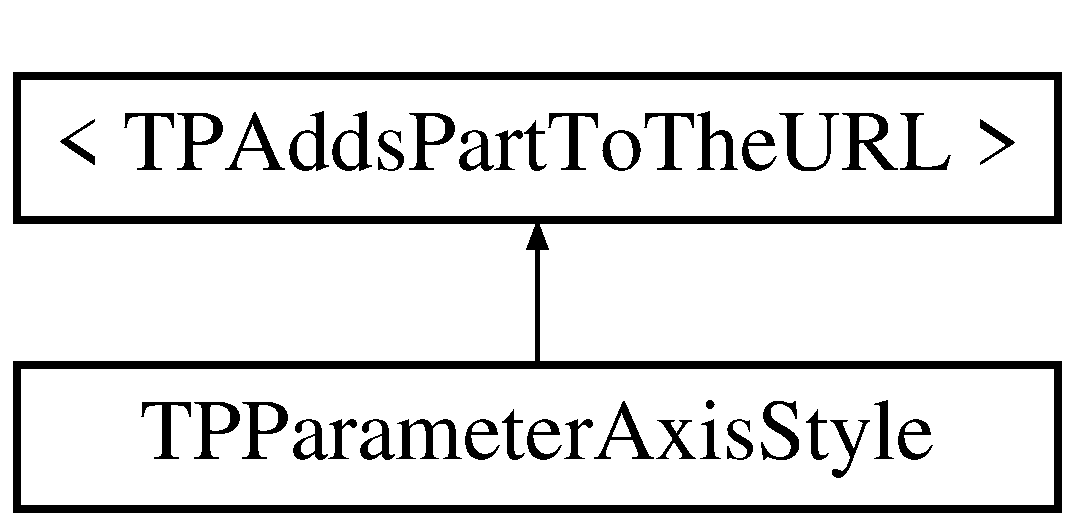
\includegraphics[height=2cm]{interface_t_p_parameter_axis_style}
\end{center}
\end{figure}
\subsection*{Static Public Member Functions}
\begin{CompactItemize}
\item 
(id) + \hyperlink{interface_t_p_parameter_axis_style_ef15fbeffb6002dde5c1128b020cb921}{parameterAxisStyleWithBottomX:topX:leftY:rightY:}
\end{CompactItemize}
\subsection*{Properties}
\begin{CompactItemize}
\item 
BOOL \hyperlink{interface_t_p_parameter_axis_style_32960050862b00747067ff4e0a665025}{bottomXAxis}
\item 
BOOL \hyperlink{interface_t_p_parameter_axis_style_023f3d06469c12184a8e87cca3a75a02}{topXAxis}
\item 
BOOL \hyperlink{interface_t_p_parameter_axis_style_78a223caf4b42242604f27c1506d25ec}{leftYAxis}
\item 
BOOL \hyperlink{interface_t_p_parameter_axis_style_1e8f22695a7b7ddb29e6355c6533d7bd}{rightYAxis}
\end{CompactItemize}


\subsection{Detailed Description}
This class is responsible for controlling which axes need to be drawn you have four axis you can draw: bottom X-axis top X-axis left Y-axis right Y-axis 

\subsection{Member Function Documentation}
\hypertarget{interface_t_p_parameter_axis_style_ef15fbeffb6002dde5c1128b020cb921}{
\index{TPParameterAxisStyle@{TPParameterAxisStyle}!parameterAxisStyleWithBottomX:topX:leftY:rightY:@{parameterAxisStyleWithBottomX:topX:leftY:rightY:}}
\index{parameterAxisStyleWithBottomX:topX:leftY:rightY:@{parameterAxisStyleWithBottomX:topX:leftY:rightY:}!TPParameterAxisStyle@{TPParameterAxisStyle}}
\subsubsection[{parameterAxisStyleWithBottomX:topX:leftY:rightY:}]{\setlength{\rightskip}{0pt plus 5cm}+ (id) parameterAxisStyleWithBottomX: (BOOL) {\em bx}\/ topX: (BOOL) {\em tx}\/ leftY: (BOOL) {\em ly}\/ rightY: (BOOL) {\em ry}}}
\label{interface_t_p_parameter_axis_style_ef15fbeffb6002dde5c1128b020cb921}


Creates and returns a new \hyperlink{interface_t_p_parameter_axis_style}{TPParameterAxisStyle} with the given values \begin{Desc}
\item[Parameters:]
\begin{description}
\item[{\em bx}]bottom X-axis \item[{\em tx}]top X-axis \item[{\em ly}]left Y-axis \item[{\em ry}]right Y-axis \end{description}
\end{Desc}
\begin{Desc}
\item[Returns:]a new initialized \hyperlink{interface_t_p_parameter_axis_style}{TPParameterAxisStyle} object \end{Desc}


\subsection{Property Documentation}
\hypertarget{interface_t_p_parameter_axis_style_32960050862b00747067ff4e0a665025}{
\index{TPParameterAxisStyle@{TPParameterAxisStyle}!bottomXAxis@{bottomXAxis}}
\index{bottomXAxis@{bottomXAxis}!TPParameterAxisStyle@{TPParameterAxisStyle}}
\subsubsection[{bottomXAxis}]{\setlength{\rightskip}{0pt plus 5cm}- (BOOL) bottomXAxis\hspace{0.3cm}{\tt  \mbox{[}read, write, assign\mbox{]}}}}
\label{interface_t_p_parameter_axis_style_32960050862b00747067ff4e0a665025}


bottom X-axis YES: draw NO: don't draw \hypertarget{interface_t_p_parameter_axis_style_78a223caf4b42242604f27c1506d25ec}{
\index{TPParameterAxisStyle@{TPParameterAxisStyle}!leftYAxis@{leftYAxis}}
\index{leftYAxis@{leftYAxis}!TPParameterAxisStyle@{TPParameterAxisStyle}}
\subsubsection[{leftYAxis}]{\setlength{\rightskip}{0pt plus 5cm}- (BOOL) leftYAxis\hspace{0.3cm}{\tt  \mbox{[}read, write, assign\mbox{]}}}}
\label{interface_t_p_parameter_axis_style_78a223caf4b42242604f27c1506d25ec}


left Y-axis YES: draw NO: don't draw \hypertarget{interface_t_p_parameter_axis_style_1e8f22695a7b7ddb29e6355c6533d7bd}{
\index{TPParameterAxisStyle@{TPParameterAxisStyle}!rightYAxis@{rightYAxis}}
\index{rightYAxis@{rightYAxis}!TPParameterAxisStyle@{TPParameterAxisStyle}}
\subsubsection[{rightYAxis}]{\setlength{\rightskip}{0pt plus 5cm}- (BOOL) rightYAxis\hspace{0.3cm}{\tt  \mbox{[}read, write, assign\mbox{]}}}}
\label{interface_t_p_parameter_axis_style_1e8f22695a7b7ddb29e6355c6533d7bd}


right Y-axis YES: draw NO: don't draw \hypertarget{interface_t_p_parameter_axis_style_023f3d06469c12184a8e87cca3a75a02}{
\index{TPParameterAxisStyle@{TPParameterAxisStyle}!topXAxis@{topXAxis}}
\index{topXAxis@{topXAxis}!TPParameterAxisStyle@{TPParameterAxisStyle}}
\subsubsection[{topXAxis}]{\setlength{\rightskip}{0pt plus 5cm}- (BOOL) topXAxis\hspace{0.3cm}{\tt  \mbox{[}read, write, assign\mbox{]}}}}
\label{interface_t_p_parameter_axis_style_023f3d06469c12184a8e87cca3a75a02}


top X-axis YES: draw NO: don't draw 

The documentation for this class was generated from the following files:\begin{CompactItemize}
\item 
TPParameterAxisStyle.h\item 
TPParameterAxisStyle.m\end{CompactItemize}
